\documentclass[12pt,]{article}
\usepackage{lmodern}
\usepackage{amssymb,amsmath}
\usepackage{ifxetex,ifluatex}
\usepackage{fixltx2e} % provides \textsubscript
\ifnum 0\ifxetex 1\fi\ifluatex 1\fi=0 % if pdftex
  \usepackage[T1]{fontenc}
  \usepackage[utf8]{inputenc}
\else % if luatex or xelatex
  \ifxetex
    \usepackage{mathspec}
  \else
    \usepackage{fontspec}
  \fi
  \defaultfontfeatures{Ligatures=TeX,Scale=MatchLowercase}
    \setmainfont[]{Times New Roman}
\fi
% use upquote if available, for straight quotes in verbatim environments
\IfFileExists{upquote.sty}{\usepackage{upquote}}{}
% use microtype if available
\IfFileExists{microtype.sty}{%
\usepackage{microtype}
\UseMicrotypeSet[protrusion]{basicmath} % disable protrusion for tt fonts
}{}
\usepackage[margin=2.54cm]{geometry}
\usepackage{hyperref}
\hypersetup{unicode=true,
            pdftitle={Impacts of Land Use on Water Quality in Minnesota},
            pdfauthor={Keith Bollt, Jake Greif, Felipe Raby-Amadori, \& Lindsay Roth},
            pdfborder={0 0 0},
            breaklinks=true}
\urlstyle{same}  % don't use monospace font for urls
\usepackage{longtable,booktabs}
\usepackage{graphicx,grffile}
\makeatletter
\def\maxwidth{\ifdim\Gin@nat@width>\linewidth\linewidth\else\Gin@nat@width\fi}
\def\maxheight{\ifdim\Gin@nat@height>\textheight\textheight\else\Gin@nat@height\fi}
\makeatother
% Scale images if necessary, so that they will not overflow the page
% margins by default, and it is still possible to overwrite the defaults
% using explicit options in \includegraphics[width, height, ...]{}
\setkeys{Gin}{width=\maxwidth,height=\maxheight,keepaspectratio}
\IfFileExists{parskip.sty}{%
\usepackage{parskip}
}{% else
\setlength{\parindent}{0pt}
\setlength{\parskip}{6pt plus 2pt minus 1pt}
}
\setlength{\emergencystretch}{3em}  % prevent overfull lines
\providecommand{\tightlist}{%
  \setlength{\itemsep}{0pt}\setlength{\parskip}{0pt}}
\setcounter{secnumdepth}{5}
% Redefines (sub)paragraphs to behave more like sections
\ifx\paragraph\undefined\else
\let\oldparagraph\paragraph
\renewcommand{\paragraph}[1]{\oldparagraph{#1}\mbox{}}
\fi
\ifx\subparagraph\undefined\else
\let\oldsubparagraph\subparagraph
\renewcommand{\subparagraph}[1]{\oldsubparagraph{#1}\mbox{}}
\fi

%%% Use protect on footnotes to avoid problems with footnotes in titles
\let\rmarkdownfootnote\footnote%
\def\footnote{\protect\rmarkdownfootnote}

%%% Change title format to be more compact
\usepackage{titling}

% Create subtitle command for use in maketitle
\providecommand{\subtitle}[1]{
  \posttitle{
    \begin{center}\large#1\end{center}
    }
}

\setlength{\droptitle}{-2em}

  \title{Impacts of Land Use on Water Quality in Minnesota}
    \pretitle{\vspace{\droptitle}\centering\huge}
  \posttitle{\par}
  \subtitle{\url{https://github.com/lhr12/HDA_Project}}
  \author{Keith Bollt, Jake Greif, Felipe Raby-Amadori, \& Lindsay Roth}
    \preauthor{\centering\large\emph}
  \postauthor{\par}
    \date{}
    \predate{}\postdate{}
  

\begin{document}
\maketitle

\newpage

\textless Arrow brackets are used for annotating the RMarkdown files.
Text within these brackets should not appear in the final version of the
PDF document\textgreater{}

\textless{}\textbf{General Guidelines}\textgreater{} \textless1. Write
in scientific style\textgreater{} \textless2.
\href{https://rmarkdown.rstudio.com/lesson-3.html}{Global options for R
chunks} should be set so that only relevant output is
displayed\textgreater{} \textless3. Make sure your final knitted PDF
looks professional. Format tables appropriately, size figures
appropriately, make sure bulleted and numbered lists appear as such,
avoid awkwardly placed page breaks, etc.\textgreater{}

\hypertarget{rationale-and-research-questions}{%
\section{Rationale and Research
Questions}\label{rationale-and-research-questions}}

\textless Write 1-2 paragraph(s) detailing the rationale for your study.
This should include both the context of the topic as well as a rationale
for your choice of dataset (reason for location, variables, etc.) A few
citations should be included to give context for your topic. You may
choose to configure autoreferencing for your citations or add these
manually.\textgreater{}

\begin{itemize}
\tightlist
\item
  Land use has a large impact on nutrient runoff into streams, lakes,
  and other water bodies
\item
  Minnesota has wide variety of land uses. Inlcudes large urban centers,
  natural lands, and agricultural area.
\item
  Nutrient management has been a challenge for states in the effort to
  control harmful algal blooms and coastal dead zones.
\item
  Understanding the causes of nutrient problems will better inform
  management strategies.
\end{itemize}

Research questions:

\begin{enumerate}
\def\labelenumi{\arabic{enumi}.}
\item
  What are the predictors of nutrients based on land use in watersheds
  in the state of Minnesota?
\item
  How do you characterize seasonal variation between the predictors of
  nutrients?
\end{enumerate}

Goals:

\begin{itemize}
\tightlist
\item
  Determine how land use, watershed size, and ecoregion explain
  variation in nutrient loading indicators.
\item
  Discern whether there a seasonal trends in nutrient loading indicators
  based on land use types, watershed size, and ecoregion.
\item
  Provide insight to inform decisions about nutrient managment practices
  based on land use types, watershed size, and ecoregion.
\end{itemize}

\textless At the end of your rationale, introduce a numbered list of
your questions (or an overarching question and sub-questions). Each
question should be accompanied by one or more working hypotheses,
inserted beneath each question.\textgreater{}

Research questions:

\begin{enumerate}
\def\labelenumi{\arabic{enumi}.}
\item
  What are the predictors of nutrients based on land use in watersheds
  in the state of Minnesota?

  Hypothesis:
\item
  How do you characterize seasonal variation between the predictors of
  nutrients?

  Hypothesis:
\end{enumerate}

\newpage

\hypertarget{dataset-information}{%
\section{Dataset Information}\label{dataset-information}}

\textless Provide information on how the dataset for this analysis were
collected, the data contained in the dataset, and any important pieces
of information that are relevant to your analyses. This section should
contain much of same information as the metadata file for the dataset
but formatted in a way that is more narrative.\textgreater{}

The data used in this analysis include data from the Lake Multi-Scaled
Geospatial and Temporal Database (LAGOSNE) and the EPA ecoregion spatial
datasets.

LAGOSNE is a collection of several data modules that contain information
on lakes in the northern United States. The modules contain data from
thousands of lakes in 17 states in the northeastern and midwestern
United States, from Missouri to Maine. The dataset includes a complete
list of all lakes bigger than 4 hectacres in the 17 state area, and
water quality data on a large number of lakes, spanning every state.

Ecoregions are used by planning managers to understand the type of land
use that occurs in different regions of the United States. There are
different levels of ecoregions. Level 1 divides North America into 15
ecological regions, while Level IV offers fine ecological resolution for
each state. This data was published by the U.S. EPA Office of Research
and Development (ORD) - National Health and Environmental Effects
Research Laboratory (NHEERL). For the purposes of our project, we
selected Level III ecoregions because they appear to offer a descriptive
narrative of the land use patterns of Minnesota without making a
`distinction without a difference'.

\textless Describe how your team wrangled your dataset in a format
similar to a methods section of a journal article.\textgreater{}

******Not included in original draft*********

\textless Add a table that summarizes your data structure (variables,
units, ranges and/or central tendencies, data source if multiple are
used, etc.). This table can be made in markdown text or inserted as a
\texttt{kable} function in an R chunk. If the latter, do not include the
code used to generate your table.\textgreater{}

\begin{longtable}[]{@{}llll@{}}
\toprule
Column.Name & Description & Units & Variable.Type\tabularnewline
\midrule
\endhead
chla & Chlorophyll a & mg/L & Dependent\tabularnewline
secchi & Secchi depth & m & Dependent\tabularnewline
IntenseUrban.pct & Percent med. and high intensity urban land cover & \%
& Independent\tabularnewline
OpenUrban.pct & Percent developed & \% & Independent\tabularnewline
Barren.pct & Percent areas of bedrock and desert pavement land cover &
\% & Independent\tabularnewline
Forest.pct & Percent deciduous & \% & Independent\tabularnewline
GrassShrub.pct & Percent areas dominated by shrubs & \% &
Independent\tabularnewline
Wetland.pct & Percent wetlands land cover & \% &
Independent\tabularnewline
Pasture.pct & Percent areas of grasses & \% & Independent\tabularnewline
RowCrop.pct & Percent cultivated crops land cover & \% &
Independent\tabularnewline
LakeIWS.Ratio & Lake surface area to watershed area ratio & N/A &
Independent\tabularnewline
Season & Early/Prime/Late & N/A & Independent\tabularnewline
Ecoregion & Level II Ecoregions & N/A & Independent\tabularnewline
\bottomrule
\end{longtable}

\newpage

\hypertarget{exploratory-analysis}{%
\section{Exploratory Analysis}\label{exploratory-analysis}}

\textless Insert exploratory visualizations of your dataset. This may
include, but is not limited to, graphs illustrating the distributions of
variables of interest and/or maps of the spatial context of your
dataset. Format your R chunks so that graphs are displayed but code is
not displayed. Accompany these graphs with text sections that describe
the visualizations and provide context for further
analyses.\textgreater{}

\textless Each figure should be accompanied by a caption, and each
figure should be referenced within the text\textgreater{}

*******code below is copied directly from originial draft, it needs to
be edited to fulfill the above requirements**************

\begin{figure}
\centering
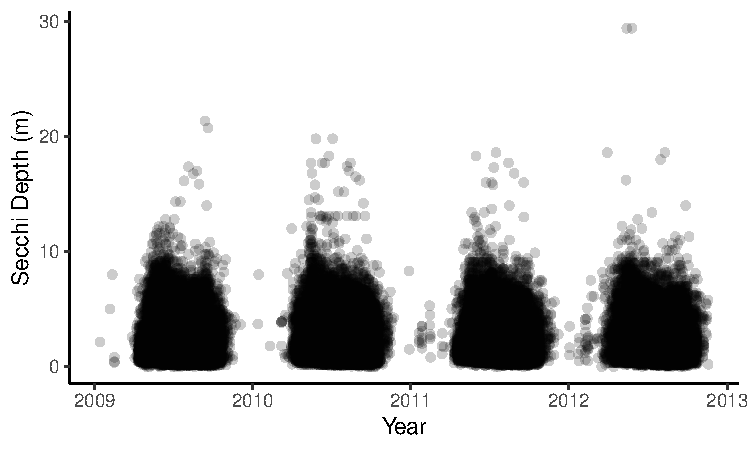
\includegraphics{Bollt_Greif_Raby_Roth_Draft_1115_files/figure-latex/Visualize_data-1.pdf}
\caption{This plot provides a sense of how secchi depth measurements are
distributed between and within years, as well as the general range of
secchi depth measurements. Sampling occurs during the middle portion of
each year, and ceases during the winter season.}
\end{figure}

\begin{longtable}[]{@{}lr@{}}
\toprule
Year & Count\tabularnewline
\midrule
\endhead
2009 & 20849\tabularnewline
2010 & 19829\tabularnewline
2011 & 18025\tabularnewline
2012 & 16924\tabularnewline
\bottomrule
\end{longtable}

\begin{figure}
\centering
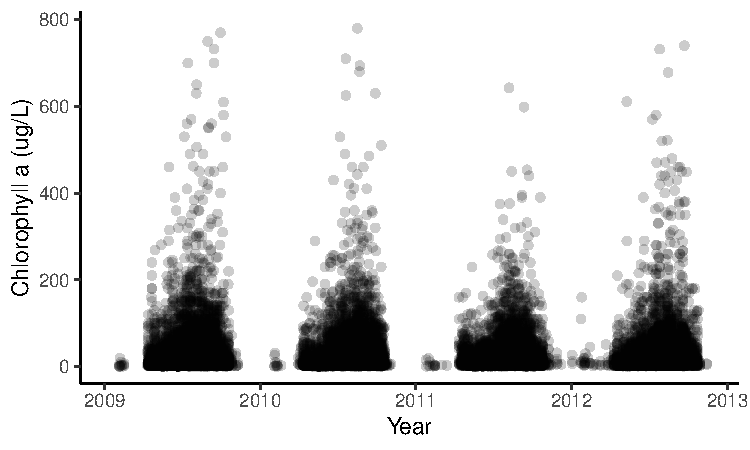
\includegraphics{Bollt_Greif_Raby_Roth_Draft_1115_files/figure-latex/unnamed-chunk-3-1.pdf}
\caption{Chlorophyll a vs.~Time. This plot provides a sense of how
chlorophyll a measurements are distributed between and within years, as
well as the general range of chlorophyll a measurements. Sampling occurs
during the middle portion of each year, and ceases during the winter
season.}
\end{figure}

\begin{longtable}[]{@{}lr@{}}
\toprule
Year & Count\tabularnewline
\midrule
\endhead
2009 & 8996\tabularnewline
2010 & 7576\tabularnewline
2011 & 6989\tabularnewline
2012 & 6206\tabularnewline
\bottomrule
\end{longtable}

\begin{verbatim}
## Reading layer `NA_CEC_Eco_Level2' from data source `C:\Users\Felipe\OneDrive - Duke University\1. DUKE\Ramos 3 Semestre\722 Hydro Data\HDA_Project_FRA\data\raw\NA_CEC_Eco_Level2.shp' using driver `ESRI Shapefile'
## Simple feature collection with 2261 features and 8 fields
## geometry type:  POLYGON
## dimension:      XY
## bbox:           xmin: -4334052 ymin: -3313739 xmax: 3324076 ymax: 4267265
## epsg (SRID):    NA
## proj4string:    +proj=laea +lat_0=45 +lon_0=-100 +x_0=0 +y_0=0 +a=6370997 +b=6370997 +units=m +no_defs
\end{verbatim}

\begin{verbatim}
##    Min. 1st Qu.  Median    Mean 3rd Qu.    Max. 
##    0.76    3.90    7.40   16.54   16.00  290.00
\end{verbatim}

\begin{verbatim}
##    Min. 1st Qu.  Median    Mean 3rd Qu.    Max. 
##    0.00    4.00    7.31   22.58   22.00  780.00
\end{verbatim}

\begin{verbatim}
##    Min. 1st Qu.  Median    Mean 3rd Qu.    Max. 
##   0.668   5.800  14.000  27.973  32.000 610.000
\end{verbatim}

\begin{verbatim}
##    Min. 1st Qu.  Median    Mean 3rd Qu.    Max. 
##   0.010   1.100   2.000   2.363   3.350  17.000
\end{verbatim}

\begin{verbatim}
##    Min. 1st Qu.  Median    Mean 3rd Qu.    Max. 
##   0.080   0.900   1.680   1.898   2.590   7.500
\end{verbatim}

\begin{figure}
\centering
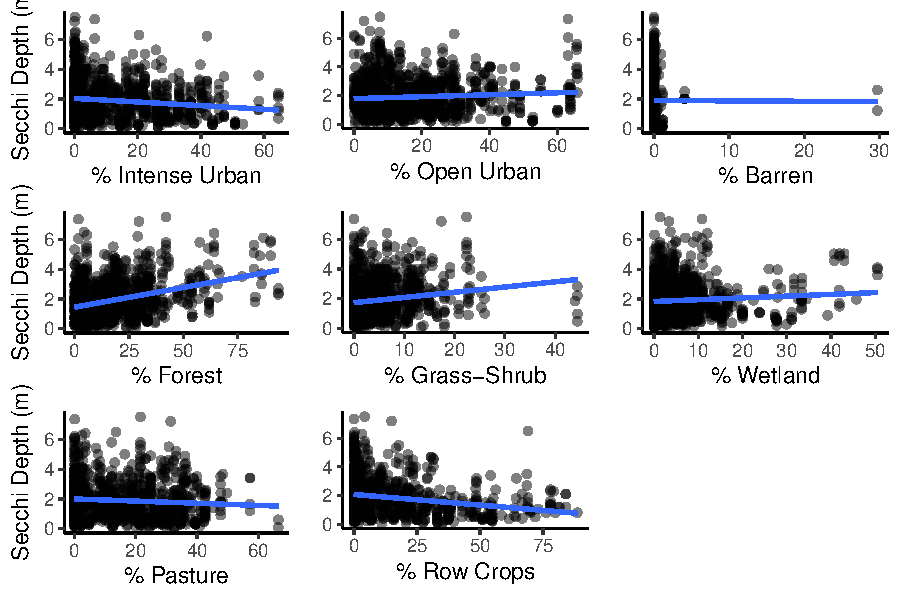
\includegraphics{Bollt_Greif_Raby_Roth_Draft_1115_files/figure-latex/unnamed-chunk-5-1.pdf}
\caption{These plots shows that there are trends in secchi depth
relative to the given land uses during the `Late Season'. The presence
of trends supports the inclusion of the above land uses in the analysis.
Note that the x-axes are on different scales.}
\end{figure}

\begin{figure}
\centering
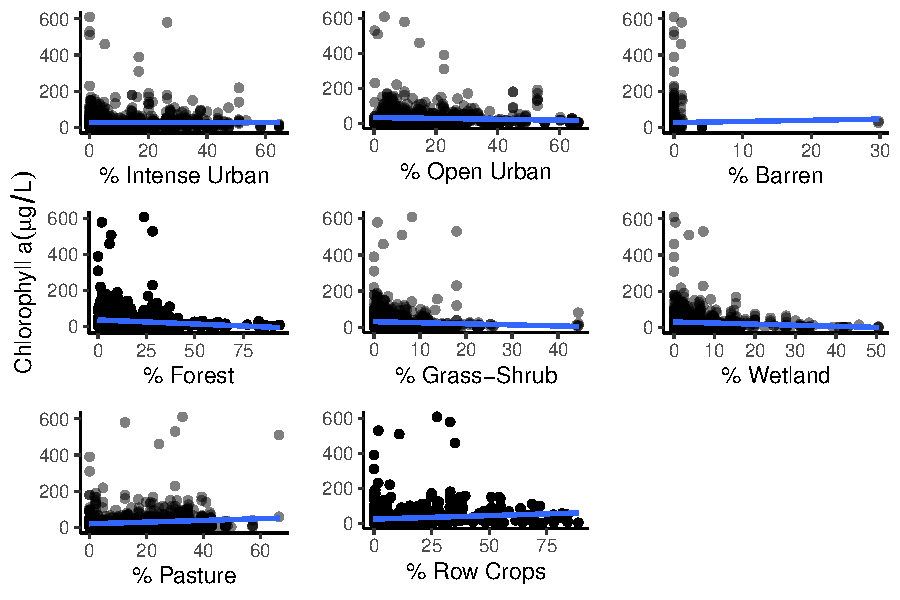
\includegraphics{Bollt_Greif_Raby_Roth_Draft_1115_files/figure-latex/unnamed-chunk-7-1.pdf}
\caption{These plots shows that there are trends in chlorophyll a
concentrations relative to the given land uses during the `Late Season'.
The presence of trends supports the inclusion of the above land uses in
the analysis. Note that the x-axes are on different scales.}
\end{figure}

Figures XX and YY explore the trends in secchi depth and chlorophyll a
by the percentage of each land use type in the late season. The late
season was chosen for exploration because it had to lowest and highest
mean secchi depth and mean chlorophyll a, respectively.

FRA Comment: Next plot main purpose is to check is we have enough data
in each ecoregion.

\begin{figure}
\centering
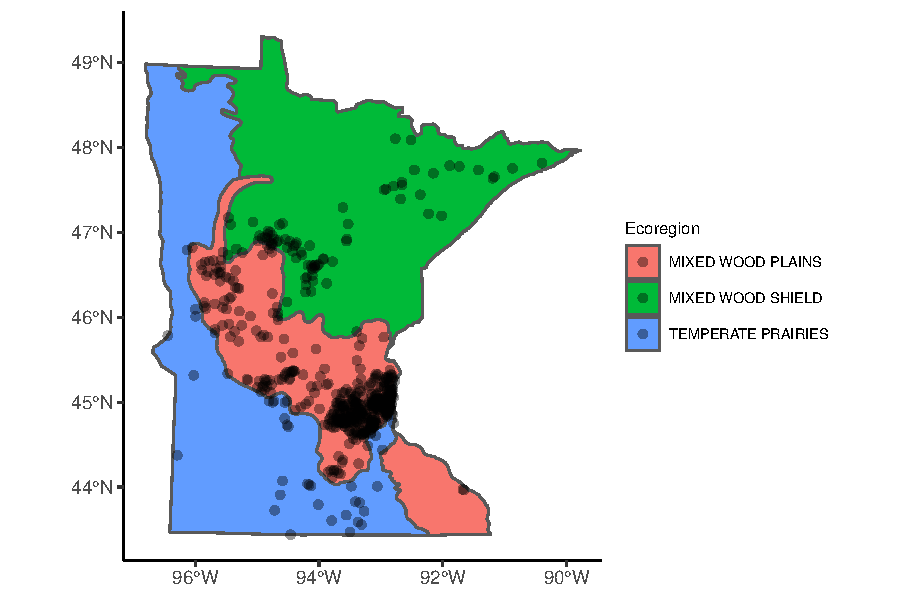
\includegraphics{Bollt_Greif_Raby_Roth_Draft_1115_files/figure-latex/summary.for.early.season-1.pdf}
\caption{These plots shows that there are trends in chlorophyll a
concentrations relative to the given land uses during the `Late Season'.
The presence of trends supports the inclusion of the above land uses in
the analysis. Note that the x-axes are on different scales.}
\end{figure}

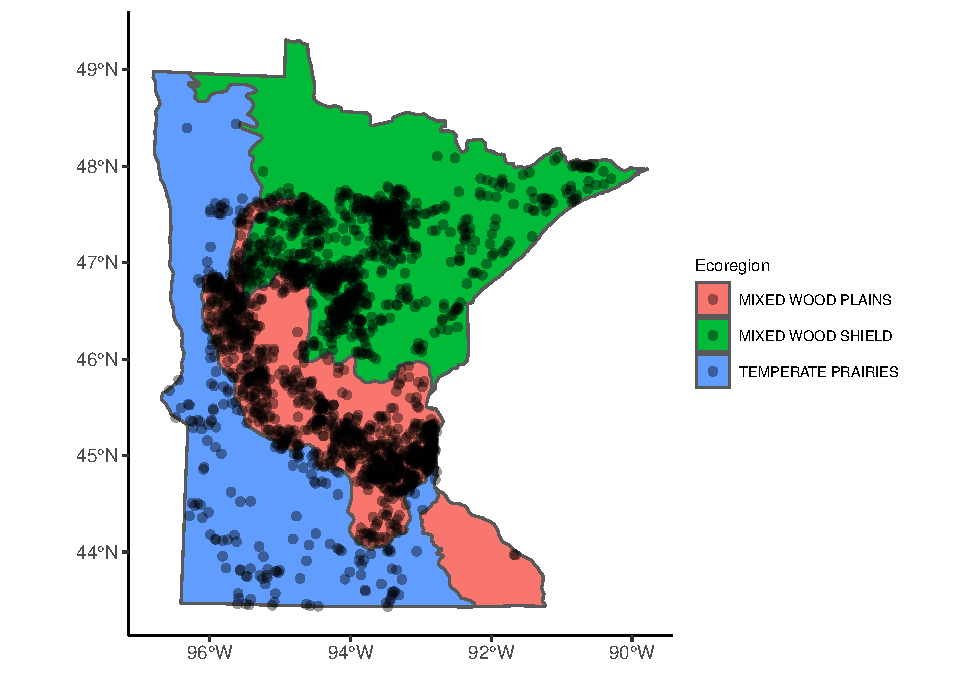
\includegraphics{Bollt_Greif_Raby_Roth_Draft_1115_files/figure-latex/summary.for.prime.season-1.pdf}

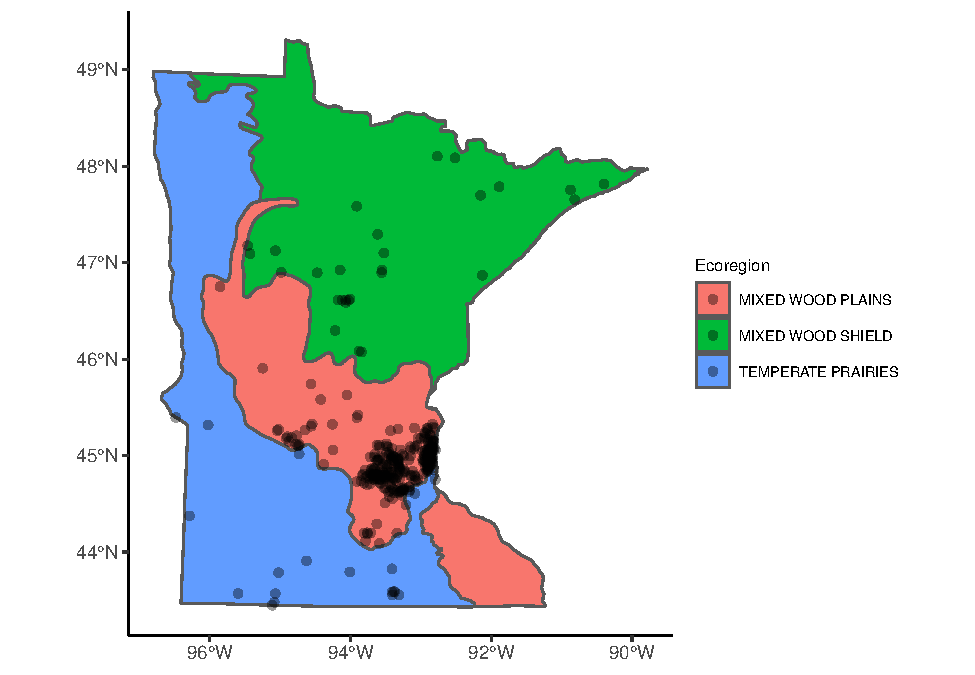
\includegraphics{Bollt_Greif_Raby_Roth_Draft_1115_files/figure-latex/summary.for.late.season-1.pdf}

FRA Comment: The next plot where the one we did for the proposal. We
have to see if we want them

\newpage

\hypertarget{analysis}{%
\section{Analysis}\label{analysis}}

\textless Insert visualizations and text describing your main analyses.
Format your R chunks so that graphs are displayed but code and other
output is not displayed. Instead, describe the results of any
statistical tests in the main text (e.g., ``Variable x was significantly
different among y groups (ANOVA; df = 300, F = 5.55, p \textless{}
0.0001)''). Each paragraph, accompanied by one or more visualizations,
should describe the major findings and how they relate to the question
and hypotheses. Divide this section into subsections, one for each
research question.\textgreater{}

\textless Each figure should be accompanied by a caption, and each
figure should be referenced within the text\textgreater{}

\begin{itemize}
\tightlist
\item
  First we will create correlation plots in order to eliminate variables
  with a correlation greater than 0.8.
\item
  Then we will run Shapiro-Wilkes tests to determine normality and the
  need for possible data transformations.
\item
  After determining the distributions of the data, then we will generate
  mixed effect linear models with chlorophyll a and secchi depth as
  response variables, land use and watershed size as fixed effects, and
  ecoregion as a random effect.
\end{itemize}

Final figures will include:

\begin{itemize}
\tightlist
\item
  6 maps of the state, each showing the relationship between land use
  and both response variables. Ecoregion will be included as a base
  layer for each map.
\item
  Scatter plots showing the strongest relationships between land use and
  the response variables.
\item
  Table showing results of linear model.
\end{itemize}

\hypertarget{question-1}{%
\subsection{Question 1: }\label{question-1}}

\hypertarget{question-2}{%
\subsection{Question 2:}\label{question-2}}

\newpage

\hypertarget{summary-and-conclusions}{%
\section{Summary and Conclusions}\label{summary-and-conclusions}}

\textless Summarize your major findings from your analyses in a few
paragraphs. What conclusions do you draw from your findings? Relate your
findings back to the original research questions and
rationale.\textgreater{}

\newpage

\hypertarget{references}{%
\section{References}\label{references}}


\end{document}
